\documentclass{IEEEcsmag}

\usepackage[colorlinks,urlcolor=blue,linkcolor=blue,citecolor=blue]{hyperref}
\expandafter\def\expandafter\UrlBreaks\expandafter{\UrlBreaks\do\/\do\*\do\-\do\~\do\'\do\"\do\-}
\usepackage{upmath,color}
\usepackage{graphicx}
\usepackage{booktabs}

\jvol{XX}
\jnum{XX}
\paper{8}
\jmonth{Month}
\jname{Computing in Science \& Engineering}
\jtitle{Computing in Science \& Engineering}
\pubyear{2026}

\setcounter{secnumdepth}{0}

\begin{document}

\sptitle{Feature Article: Research Software and Tools}

\title{Code-Hosting Platforms as Research Infrastructure: GitHub, GitLab and Bitbucket Scored Against Sixty-Two Criteria}

\author{Telmo Miguel-Medina}
\affil{Electromechanical Engineering Department, University of Burgos, Burgos, 09001, Spain}

\markboth{FEATURE ARTICLE}{FEATURE ARTICLE}

\begin{abstract}\looseness-1
Researchers are told to manage projects on a code-hosting platform, rarely which one or why. This article scores GitHub, GitLab and Bitbucket against fifteen research-management requirements split into 62 testable criteria, on free plans, from vendor documentation. GitHub scores highest (2.75 of 3), then GitLab (2.55), which holds five capabilities behind paid plans; Bitbucket alone falls to 1.76 after removing its issue tracker in 2026, and recovers with Jira and Confluence (2.48), the only configuration with a native decision record. Five AI assistants re-scored the sheet independently: agreement was moderate (Krippendorff's alpha 0.54). Every reading puts Bitbucket alone last and finds the code hosts weakest on planning, research questions and decisions, but the order of the other three is not stable. Eleven criteria are native nowhere in my scoring; the second readings confirm two.
\end{abstract}

\maketitle

\chapteri{A} research group that wants to keep its questions, plans, decisions, code, data and manuscripts in one traceable place is usually pointed to the tool its programmers already use. A companion article derives, from the literature and without reference to any tool, fifteen requirements for managing the research process, each with expected capabilities that can be checked.\textsuperscript{1} This article does the checking.

There is no shortage of encouragement. Tutorials and ``ten simple rules'' papers explain how Git and GitHub support versioned, collaborative work,\textsuperscript{2,3} and reports from ecology and from wet laboratories describe groups that run their whole project there.\textsuperscript{4,5} But this literature is case-based and about one platform, and studies that mine repositories warn that much real use is shallow.\textsuperscript{6} A researcher choosing a platform, or a student being taught to use one, gets a recommendation without the reasoning behind it: which requirement a feature meets, how well, and what it costs.

So I ask three questions. How far do the three platforms that dominate code hosting (GitHub, GitLab and Bitbucket) meet each requirement, capability by capability? Where does the answer depend on paying? And what is missing from all of them? The method matters as much as the result, because it is meant to be repeated: every score in this article can be traced to a written test, a named feature and, where I verified it, a page of vendor documentation.

\section{HOW I SCORED THE PLATFORMS}

\emph{The instrument.} The fifteen requirements come with 62 expected capabilities, between three and six each.\textsuperscript{1} I used them unchanged and wrote one test per capability. For decision traceability, for example, the five tests are: a decision can be recorded as a distinct type of record; the record has structured places for rationale and alternatives; it carries the date of the decision; it names who took part; and it links to the artifacts the decision affects.

\emph{What was scored.} The context is an open research project run by a small group with no budget for tooling: GitHub Free with an organization account and a public repository, GitLab.com Free with a public project, and Bitbucket Cloud Free with a public repository. A fourth configuration was forced by events. In August 2026 Bitbucket Cloud removed its native issue tracker and wiki and directed users to its sister products, so I scored Bitbucket twice: alone, and together with the free plans of Jira and Confluence. Only vendor features count. Third-party applications are excluded, with the one exception the requirements themselves name: an external archive that assigns persistent identifiers.

\emph{The scale.} Each capability receives a score from 0 to 3. A 3 means \emph{native}: the platform ships a feature that performs the capability as tested, with no convention imposed by the team. A 2 means \emph{by convention}: achievable with platform features, but through a generic object the team configures or a rule the platform neither models nor enforces. A 1 means \emph{marginal}: a fragment of the capability, or free text with no structure. A 0 means \emph{absent}: another product is needed. Each cell also has a second score for the vendor's highest paid plan, so that capabilities held behind a price are visible.

\emph{Aggregation.} A requirement's score is the mean of its capability scores, labeled Direct at 2.5 or above, Partial at 1.5 or above, Limited at 0.5 or above, and Not supported below that. Because a mean can hide one missing capability, I also report a stricter reading in which a requirement is only as supported as its weakest capability. Finally, taking the best score any configuration reaches for each capability gives a best-of-breed profile, and the capabilities that even that profile does not meet natively are the residual gaps.

\emph{Evidence.} This is a documentary evaluation. Scores were assigned from vendor documentation, with the assistance of a large language model, and each of the 248 cells records the feature that justifies it. For 72 cells, those where plans differ or where features changed recently, the score was verified against the vendor's own pages on 8 October 2026 and the source is logged. No configuration was exercised in a live project for this purpose. I call these the reference scores.

\emph{A second reading.} To learn how much of the result depends on one reading of the scale, the blank rating sheet (the 62 tests, the four configurations, the scale and its two worked examples, but none of my scores or evidence) was completed independently by five AI assistants on 9 October 2026. They are not human raters and I do not present their agreement as inter-rater reliability in the usual sense; no person other than the author has scored the sheet. What the five sheets can show is which conclusions survive when someone else applies the same rubric, and which do not. I report exact agreement, agreement within one point, linearly weighted kappa for each pair, and Krippendorff's alpha for ordinal data across all six readings. Three topics the scores do not isolate (mandatory review before integration, runners, and the path to a citable output) are examined separately. The criteria, the scores with their evidence, the verification log and the script that produces every number here are in the public study repository (see Acknowledgments).

\section{WHAT THE PLATFORMS COVER}

Table~\ref{tab:support} gives the result. On free plans GitHub has the highest mean, 2.75 of 3, with eleven requirements Direct and four Partial; 48 of its 62 capabilities are native and none is absent. GitLab follows at 2.55, with eight Direct and seven Partial and 39 native capabilities. Bitbucket alone scores 1.76: with no issue tracker it has nothing to register a task in, so task management is Not supported and five further requirements are Limited. With Jira and Confluence beside it, Bitbucket recovers to 2.48, with ten Direct and five Partial. Figure~\ref{fig:heatmap} shows the 62 capability scores behind these means. A later section tests them against five independent readings of the same sheet; the gap between Bitbucket alone and the rest survives that test, and the order of the other three does not.

\begin{table*}[t]
\caption{Support for the fifteen research-management requirements on free plans: mean capability score (0--3) and label (D Direct, P Partial, L Limited, N Not supported). $^\star$ marks the requirements that are highly important but weakly covered in the literature.\textsuperscript{1} ``Best'' takes, for each capability, the highest score any configuration reaches.}\label{tab:support}
\tablefont
\setlength{\tabcolsep}{4pt}
\begin{tabular*}{\textwidth}{@{\extracolsep{\fill}}p{24pt}p{146pt}<{\raggedright}rrrrr@{}}
\toprule
ID& Requirement& GitHub& GitLab& Bitbucket& Bitbucket + Jira + Confl.& Best\\
\colrule
RM1$^\star$& Research planning and roadmap& 2.50 D& 2.00 P& 0.50 L& 2.50 D& 2.50 D\\
RM2$^\star$& Research-question management& 2.33 P& 1.67 P& 1.33 L& 2.67 D& 2.67 D\\
RM3& Task management& 3.00 D& 2.33 P& 0.00 N& 3.00 D& 3.00 D\\
RM4& Documentation& 3.00 D& 2.75 D& 2.50 D& 2.75 D& 3.00 D\\
RM5$^\star$& Decision traceability& 2.40 P& 2.40 P& 1.20 L& 2.80 D& 2.80 D\\
RM6& Collaboration and contribution tracking& 3.00 D& 2.75 D& 2.50 D& 2.50 D& 3.00 D\\
RM7& Communication& 3.00 D& 3.00 D& 1.00 L& 3.00 D& 3.00 D\\
RM8& Version control& 2.80 D& 2.80 D& 2.80 D& 2.80 D& 2.80 D\\
RM9& Artifact management and integration& 2.25 P& 2.25 P& 2.25 P& 2.00 P& 2.25 P\\
RM10& Provenance and artifact linkage& 2.25 P& 2.25 P& 1.50 P& 2.25 P& 2.25 P\\
RM11& Transparency& 3.00 D& 3.00 D& 2.00 P& 2.00 P& 3.00 D\\
RM12& Reproducibility support& 2.75 D& 2.75 D& 2.50 D& 2.50 D& 2.75 D\\
RM13& Automation& 3.00 D& 3.00 D& 2.75 D& 2.75 D& 3.00 D\\
RM14& Output management and identification& 3.00 D& 2.25 P& 1.25 L& 1.75 P& 3.00 D\\
RM15& Governance and sustainability& 3.00 D& 3.00 D& 2.25 P& 2.00 P& 3.00 D\\
\colrule
& Mean, all fifteen& 2.75& 2.55& 1.76& 2.48& 2.80\\
& Mean, RM1, RM2 and RM5& 2.41& 2.02& 1.01& 2.66& 2.66\\
& Mean on the highest paid plan& 2.75& 2.67& 1.79& 2.55& \\
\botrule
\end{tabular*}
\end{table*}

\begin{figure*}[t]
\centerline{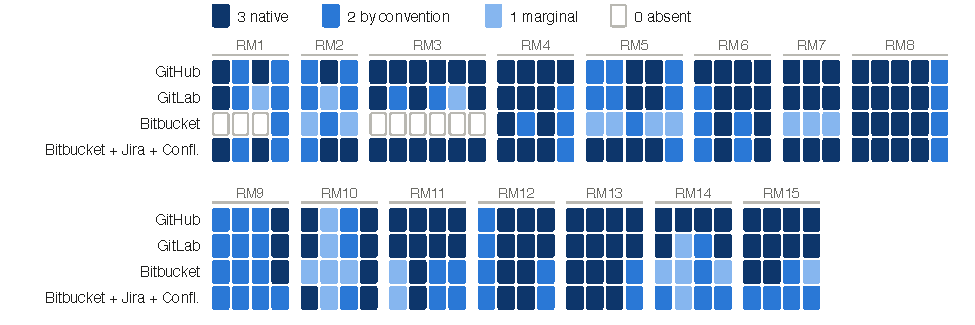
\includegraphics[width=\textwidth]{fig_heatmap.pdf}}
\caption{Scores for all 62 capabilities on free plans, grouped by requirement (RM1 to RM15, named in Table~\ref{tab:support}). Each column is one capability; within a requirement the capabilities are in the order of the published criteria sheet.}\label{fig:heatmap}
\end{figure*}

Two patterns run across the table. First, every configuration is strongest where research looks like software development. Version control, automation, reproducibility support and review-based collaboration are Direct everywhere, and differ only in quotas. Second, the three requirements the companion article singles out as important and neglected (planning, research-question management and decision traceability) score lower than the rest on GitHub (2.41 against 2.84), on GitLab (2.02 against 2.68) and on Bitbucket alone (1.01 against 1.94). None of the three code hosts ships an object for a research question or a decision; each offers a generic issue that a team can configure to stand in for one.

The exception is instructive. With Jira and Confluence, Bitbucket scores \emph{higher} on those three requirements (2.66) than on the others (2.44), and higher than GitHub. The reason is not the code host but the documentation and tracking tools beside it: Confluence ships a decision record with fields for background, options considered, outcome, owner and contributors, and keeps a decision log for the space automatically; Jira links issues with typed, configurable relationships and shows the old and new wording of any edited field. The same configuration is the weakest on transparency, because neither Jira nor Confluence can be opened to the public on a free plan.

The stricter reading sharpens the ranking of the reference scores without reversing it. Counting a requirement only when every one of its capabilities is native, GitHub fully meets eight requirements, GitLab four, the three-product Atlassian configuration two, and Bitbucket alone none. No configuration is native throughout on planning, question management, decision traceability, version control (large files are quota-bound everywhere), artifact management, provenance or reproducibility support.

\section{WHY A RATING IS WHAT IT IS}

A rating is only useful if a reader can see how it was reached and disagree with it. Table~\ref{tab:example} opens up one requirement, decision traceability, to show what lies behind a line of Table~\ref{tab:support}.

\begin{table*}[t]
\caption{The five capabilities behind one requirement, decision traceability (RM5), with the score and the evidence for each configuration. All 62 capabilities are documented this way in the study repository.}\label{tab:example}
\tablefont
\setlength{\tabcolsep}{4pt}
\begin{tabular*}{\textwidth}{@{\extracolsep{\fill}}p{84pt}<{\raggedright}p{98pt}<{\raggedright}p{78pt}<{\raggedright}p{62pt}<{\raggedright}p{96pt}<{\raggedright}@{}}
\toprule
Capability tested& GitHub& GitLab& Bitbucket& Bitbucket + Jira + Confluence\\
\colrule
A decision is a distinct type of record& 2: issue type or discussion category configured for decisions& 2: issue with a label or template& 1: a file in the repository& 3: Confluence decision record with automatic log\\[2pt]
Structured places for rationale and alternatives& 2: issue forms and issue fields configured by the team& 2: description template, free text& 1: file template& 3: template with background, options and outcome\\[2pt]
Date of the decision& 3: timestamps on the record& 3: timestamps on the record& 2: commit date of the file& 3: timestamps and due date\\[2pt]
Who took part& 3: assignees and participants& 3: assignee and participants& 1: commit author only& 3: owner, contributors, informed parties\\[2pt]
Links to affected artifacts& 2: cross-references, not typed& 2: cross-references, not typed& 1: free-text references& 2: smart links, not typed\\
\colrule
Mean and label& 2.40 Partial& 2.40 Partial& 1.20 Limited& 2.80 Direct\\
\botrule
\end{tabular*}
\end{table*}

Read down the GitHub column and the Partial label explains itself: the platform timestamps and attributes anything, but it has no notion of a decision, so the first, second and fifth capabilities rest on what the team agrees to do. Read across the first row and the difference between a 2 and a 3 is concrete: a configured issue type is a convention the platform tolerates, a decision record with its own log is a feature the platform maintains. A reader who thinks a configured issue type deserves a 3 can change that one cell and see what happens to the mean. That is the point of scoring capabilities rather than requirements. On this requirement the five AI rating sheets mostly agree with the table: every one scores the first capability 2 for GitHub and for GitLab, and three of the five score it 3 for the Atlassian configuration. The other two score it 2.

\section{DO THE SCORES SURVIVE A SECOND READING?}

Only in part. The five AI rating sheets supply 1{,}239 scores (one cell was left undetermined). Each sheet gives the same score as the reference in 63 to 69\% of the 248 cells and a score within one point in 88 to 96\%; weighted kappa against the reference runs from 0.34 to 0.54, and the sheets agree with one another no better (0.34 to 0.63). Krippendorff's alpha across the six readings is 0.54. That is moderate agreement, below the 0.67 usually asked of a coding scheme before even tentative conclusions are drawn from it. The numbers in Table~\ref{tab:support} should be read with that in mind: the second decimal carries no information, and neither does a difference of a few tenths between two configurations.

The disagreement has a direction and a location. The sheets are more generous than the reference, by 0.02 to 0.27 points on average; their median is higher than the reference in 53 cells and lower in 18. And they disagree far more about some configurations than others (Figure~\ref{fig:raters}): on GitHub a sheet matches the reference in 77 to 89\% of cells, on Bitbucket alone in 41 to 53\%.

\begin{figure*}[t]
\centerline{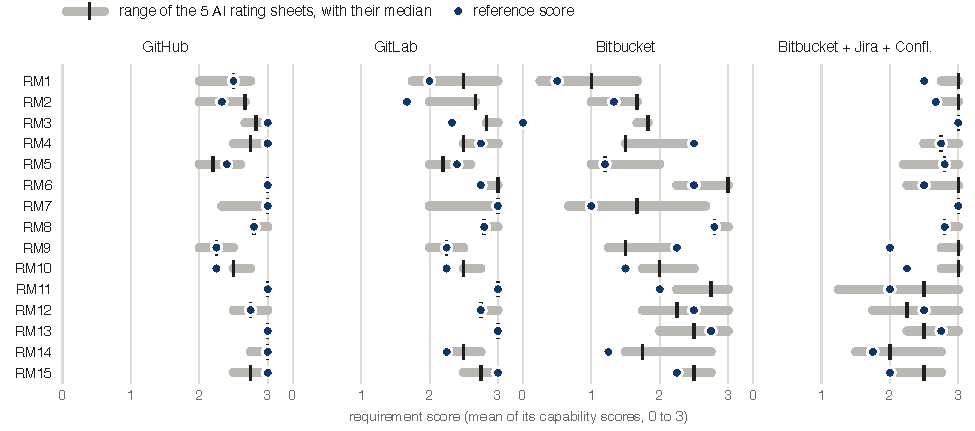
\includegraphics[width=\textwidth]{fig_raters.pdf}}
\caption{The reference score for each requirement against the five AI rating sheets. The bar spans the lowest and highest sheet and the tick is their median. Requirements RM1 to RM15 are named in Table~\ref{tab:support}.}\label{fig:raters}
\end{figure*}

Part of that gap is not a difference of judgment. All five sheets score Bitbucket alone as if it still had an issue tracker: all five give it full marks for assigning a task to a person, a capability the vendor removed in August 2026. Four of the five give GitLab's free plan full marks for mandatory review, although GitLab's documentation says that approvals there are optional and do not prevent merging. On the 72 cells I had verified against dated vendor pages, a sheet matches the reference in only 46 to 54\% of cases; on the 176 I had not, in 70 to 76\%. The disagreement concentrates exactly where the platforms changed recently, which is where a rater working from what it already knows is most likely to be out of date. On those cells I keep the reference score, and the episode is its own warning about scoring platforms from memory, whoever does it.

The rest is judgment, and there the sheets have a point. In 14 unverified cells all five sheets fall on the same side of the reference, and eight of those raise the Atlassian configuration, among them on tracking objectives, on linking a decision to what it affects, on reusable project structure, on references to artifacts held elsewhere, on reaching everything from one place, and on linking items across stages. I scored Jira and Confluence more strictly than five other readers of the same rubric. If the reference is kept where it was verified and the median of the sheets is taken everywhere else, the means become 2.77 for GitHub, 2.72 for Bitbucket with Jira and Confluence, 2.57 for GitLab and 1.77 for Bitbucket alone: the Atlassian configuration moves from third place to second.

\begin{table}[t]
\caption{Mean over the fifteen requirements in each reading of the sheet. S1 to S5 are the AI rating sheets; the last row takes their median cell by cell. Bitb.+J+C is Bitbucket with Jira and Confluence. Bold marks the highest mean in each reading.}\label{tab:readings}
\tablefont
\setlength{\tabcolsep}{3pt}
\begin{tabular*}{\columnwidth}{@{\extracolsep{\fill}}lrrrr@{}}
\toprule
Reading& GitHub& GitLab& Bitb.& Bitb.+J+C\\
\colrule
Reference& \textbf{2.75}& 2.55& 1.76& 2.48\\
S1& 2.55& \textbf{2.65}& 1.87& 2.47\\
S2& 2.61& 2.65& 2.11& \textbf{2.85}\\
S3& 2.86& 2.74& 2.08& \textbf{2.87}\\
S4& \textbf{2.83}& 2.71& 1.99& 2.67\\
S5& \textbf{2.74}& 2.72& 2.17& 2.66\\
\colrule
Median, S1--S5& \textbf{2.78}& 2.73& 2.01& 2.76\\
\botrule
\end{tabular*}
\end{table}

Table~\ref{tab:readings} separates what is robust from what is not. Three things hold in all six readings. Bitbucket alone is last, by a wide margin. On GitHub, on GitLab and on Bitbucket alone, planning, question management and decision traceability score below the other twelve requirements. And no reading gives any code host on its own a native decision record, while the reference and three of the five sheets give one to the Atlassian configuration; that configuration scores higher on the three upstream requirements than on the rest in five readings of six. GitHub's lead on citation is equally stable: four sheets of five score its use of citation metadata as native and none does so for any other configuration.

The order of the other three configurations does not hold. GitHub has the highest mean in three readings, the Atlassian configuration in two and GitLab in one, and in the median of the sheets the three are separated by 0.05. Requirement labels are no firmer: 40 of the 60 labels in Table~\ref{tab:support} are unchanged when the median of the sheets replaces the reference. The honest summary is that GitHub, GitLab and Bitbucket with Jira and Confluence cover the requirements to a similar overall degree, with different strengths, and that Bitbucket alone does not.

\section{WHAT COSTS MONEY}

For a public project GitHub's score does not change with the plan: none of the 62 capabilities improves by paying. The other configurations do change. On GitLab five capabilities rise on a paid plan: the roadmap view, blocking links between tasks, comparison of earlier wordings of an issue, intermediate task statuses, and mandatory approval of merge requests; its mean moves from 2.55 to 2.67. On Bitbucket two rise, both about enforcement: blocking a merge until approvals are given and until checks pass. With Jira and Confluence four rise, the same two plus configurable permissions and public viewing of issues.

The pattern matters for a research group. What GitLab and Bitbucket reserve for paying customers is not capacity but the planning and control features a research project needs most: the plan's timeline, the dependency between tasks, the history of a question's wording, and the guarantee that a change was reviewed. A group that chooses one of them on a free plan gets a narrower tool than the feature list suggests, and the score on the highest plan (bottom row of Table~\ref{tab:support}) shows how much narrower.

\section{WHO ALREADY WORKS THIS WAY}

Evidence that research groups manage work on these platforms exists, and it is lopsided. In a bibliometric corpus of research-process literature,\textsuperscript{1} 4{,}049 works were retrieved by queries that name no platform; 73 of them mention GitHub in their title or abstract, 12 mention GitLab and three mention Bitbucket. The share of scholarly articles that link to GitHub has risen steadily.\textsuperscript{7} Of fifteen primary studies of version control in research that I examined, ten document Git with GitHub, none documents GitLab or Bitbucket, and the remainder are tool-independent, concern Git alone, or study a data repository.

What those studies show is use for execution: versioning, review, task tracking and automation.\textsuperscript{2--5} The strongest cases are two journals that run their entire editorial process on GitHub, using issues for open peer review and pull requests for submissions.\textsuperscript{8,9} Tool-independent guidance asks for the same practices without naming a host,\textsuperscript{10,11} and one community reports using the platform to develop and version data standards.\textsuperscript{12} None of these reports describes registering research questions or logging decisions on the platform, which is consistent with Table~\ref{tab:support}: groups use what the platforms do natively.

\section{REVIEW, RUNNERS AND THE ROAD TO A CITABLE OUTPUT}

Three matters deserve a closer look than a mean allows (Table~\ref{tab:probes}).

\begin{table*}[t]
\caption{Three matters examined outside the scores, on free plans unless stated.}\label{tab:probes}
\tablefont
\setlength{\tabcolsep}{4pt}
\begin{tabular*}{\textwidth}{@{\extracolsep{\fill}}p{112pt}<{\raggedright}p{102pt}<{\raggedright}p{102pt}<{\raggedright}p{102pt}<{\raggedright}@{}}
\toprule
Question& GitHub& GitLab& Bitbucket\\
\colrule
\multicolumn{4}{@{}l}{\emph{Review before integration}}\\
Can approval be required at no cost?& Yes, on public repositories& No: approvals do not prevent merging& No: unmet checks only warn\\
Can it be required on a paid plan?& Yes& Yes, Premium& Yes, Premium\\
Can passing checks be required at no cost?& Yes, on public repositories& Yes& No, Premium only\\[3pt]
\multicolumn{4}{@{}l}{\emph{Runners}}\\
Hosted compute at no cost& Unlimited on standard runners for public repositories& 400 minutes a month& 50 minutes a month\\
Self-hosted runners& Yes& Yes& Yes; pricing changed in 2026\\[3pt]
\multicolumn{4}{@{}l}{\emph{Path to a citable output}}\\
Release with notes and files& Yes& Yes& Tags only\\
Archive with a persistent identifier& Native Zenodo integration& Manual deposit or a script in a pipeline& Manual deposit\\
Citation metadata used by the platform& Citation file read and displayed& File stored, not interpreted& File stored\\
Anyone can open an issue, as a software journal requires& Yes& Yes& Doubtful since the tracker was removed\\
\botrule
\end{tabular*}
\end{table*}

\emph{Review before integration.} All three platforms have the object: a proposed change that others comment on, line by line, and approve. For research this is internal peer review of an analysis, a protocol or a manuscript section before it enters the record. The difference is whether review can be made a rule. On a free plan only GitHub lets a public project refuse a merge until someone else has approved it; GitLab and Bitbucket record the approval but let the author merge without it, and sell the enforcement. A solo researcher loses nothing. A group that wants to say every change to the analysis was seen by a second person can only say it, at no cost, on one platform. This is a point on which the AI rating sheets and the vendors' documentation part ways: most of the sheets credit all three platforms with mandatory review, and the pages cited in the verification log say otherwise for GitLab and Bitbucket on free plans.

\emph{Runners.} Automation needs a machine to run on. Each platform offers hosted runners and lets a group register its own, which matters when an analysis needs institutional data, a licensed program or a large machine. The free hosted allowance differs by two orders of magnitude, from 50 minutes a month to unlimited for public repositories, so on Bitbucket and, for heavy pipelines, on GitLab a self-hosted runner is less an option than a necessity. Scheduled runs, which make it possible to re-execute an analysis periodically and learn when it stops reproducing, are available on all three.

\emph{The road to a citable output.} A research output should end as a named version, archived, with a persistent identifier and citation metadata. GitHub and GitLab have a release object; Bitbucket has tags. Only GitHub is connected natively to an archive that mints a DOI for each release, and only GitHub reads a citation file and offers the citation to visitors; on GitLab the same result takes a manual deposit or a script in a pipeline. For software, a further step is review by a journal that publishes it as a paper with a DOI. The best-known such journal accepts software hosted anywhere the code can be browsed and anyone can open an issue without approval or payment, and it conducts the review itself in GitHub issues regardless of where the software lives.\textsuperscript{8} A project hosted only on Bitbucket, which no longer has an issue tracker of its own, probably no longer meets that condition; this is my inference from the two published policies, not a statement by the journal.

\section{HOW TO SET IT UP}

The companion article orders the requirements into three adoption tiers.\textsuperscript{1} On any of these platforms the tiers translate into the same sequence of steps; only the names of the features change.

\emph{Record.} Create the repository with a documentation folder on the first day, before there are data. Keep the plan, the research questions and a numbered decision log as text files, or register questions and decisions as issues of a type reserved for them, with a form that asks for rationale and alternatives. On the Atlassian configuration use the decision record instead. Name every state you report with a tag.

\emph{Coordinate.} Turn the plan into milestones and a board. Make each task an issue with an owner; mark what blocks what where the platform allows it. Propose every substantive change as a pull or merge request and have someone else review it; where the plan permits, protect the main branch so that this is enforced rather than promised.

\emph{Connect and release.} Adopt one rule above all: every commit, request and issue names the question, decision or task it serves. That rule is what turns separate features into a traceable chain, and no platform enforces it, so write a small automated check that does. Add a pipeline that regenerates tables and figures and runs on a schedule. Publish releases, deposit each in an archive that assigns a DOI, and keep a citation file in the repository. A repository template that implements these steps, with every file mapped to the requirement it serves, is part of the study repository.

\section{THE TOOL NOBODY HAS BUILT}

Taking the best score any configuration reaches for each capability gives a mean of 2.80, barely above GitHub alone, and thirteen Direct requirements. The components of that profile come from different places. GitHub alone reaches the best score on four capabilities: mandatory review at no cost, the archive that assigns identifiers, citation metadata the platform uses, and project metadata it interprets. The Atlassian tools alone reach it on three: the decision record, its structured rationale, and typed links from a question to what addresses it. A platform that combined GitHub's openness and publication path with Confluence's decision record and Jira's typed links would lead on every requirement.

Even that combination leaves eleven of the 62 capabilities met natively by no one in the reference scores. Four concern the upstream process: registering a research question as an object of its own, tracking objectives, retrieving earlier versions of the plan, and typed links from a decision to the artifacts it affects. Two concern provenance: linking items across stages of the project, and querying the chain from a result back to its question, the lowest-scoring capability of all, which every platform leaves to manual navigation. The rest concern artifacts: a defined project structure, classification of artifacts by type, structured references to artifacts held elsewhere, capture of the computational environment, and large files.

How long that list is depends on how strictly \emph{native} is read, and it is the least robust result in this article. The five AI rating sheets find between one and ten capabilities with no native support, not eleven, and a majority of them confirm only two of mine: versioning large files and capturing the computational environment. They credit Jira's typed links and Confluence's templates and smart links with meeting natively what I scored as convention, and they accept a file under version control as a retrievable history of the plan. They do agree with the reference on what the object is not: none of the five finds a native record for a research question, or for a decision, on any code host. The firm part of the list is therefore short (data and environments), and the part that matters most for the argument (questions, decisions and the links between them) is firm for GitHub, GitLab and Bitbucket but contested for the Atlassian tools.

For vendors, the list is still a specification. A research question and a decision as first-class records, with revision history and typed links, would be a small addition to an issue tracker; a query that walks the links from a release back to the questions it answers would turn cross-references that already exist into provenance. For research groups, the list says where discipline has to substitute for tooling, whatever platform they choose.

\section{WHAT THIS EVALUATION CAN AND CANNOT SAY}

The main limitation is that this is a documentary evaluation. Scores describe what vendor documentation says a platform does, not what a research group experiences when it tries. Fewer than a third of the cells were verified against documentation on a stated date, and none was tested in a live project; some scores for Jira and Confluence in particular rest on knowledge of the products that I have not re-checked, and those are the scores the second readings most often dispute. Usability, which decides adoption outside computational fields, is not measured at all.

Second, no person other than the author has scored the sheet. The five second readings came from AI assistants, which share training data with one another and with the model that helped produce the reference scores, so their agreement is not independent evidence in the way five human experts' would be; and, as shown above, they were out of date on precisely the facts that changed in 2026. Their disagreement is informative all the same. An alpha of 0.54 means the boundary between \emph{native} and \emph{by convention} is not yet drawn sharply enough for two readers to place it in the same spot, and the conclusions that depend on that boundary (the order of the three leading configurations, the labels, the count of residual gaps) should be treated as provisional. The 14 unverified cells where all five sheets oppose the reference are listed in the repository as the first candidates for adjudication, and a rating by human users of each platform remains the missing step. The sheet is published so that anyone can supply it.

Third, the mean flatters. It treats capabilities as equally important and lets strong ones compensate for weak ones; the stricter reading corrects for this in one direction only. Governance is a clear case: it scores 3.00 on two platforms because its four listed capabilities are all things a platform can do, while the funding and staffing that decide whether a project survives are outside any platform.

Fourth, the result has a date. Within the fourteen months before this evaluation one platform added task dependencies and structured issue fields and another removed its issue tracker altogether. The scores are a snapshot of October 2026; the instrument and the script are what should last. Finally, three platforms and one vendor's companion products are not the whole field: self-hosted and community-run forges, and tools built for research rather than software, were not scored.

\section{CONCLUSION}

Scored against 62 capabilities derived from the research-management literature, on the free plans a small open project would use, GitHub covers the most in my scoring (2.75 of 3), GitLab is close behind (2.55) but keeps planning and enforcement features for paying customers, and Bitbucket with Jira and Confluence (2.48) offers the only native decision record of the four configurations, at the cost of public visibility. Five independent readings of the same sheet by AI assistants agree with those scores only moderately (alpha 0.54) and do not reproduce that order: among the three, each comes first in at least one reading, and the differences between them are smaller than the disagreement between readers. A group choosing among them should choose on the specific capabilities it needs, not on the mean. Two of those are documented by the vendors: only GitHub can require review before integration at no cost, and only GitHub connects natively to an archive that assigns a DOI.

What every reading agrees on is narrower and firmer. Bitbucket on its own is no longer a place to manage a project since it removed its issue tracker. The code hosts are strongest where research resembles software development and weakest on the research question, the plan and the decision, for which none ships an object of its own. How many capabilities are native nowhere depends on the reader, from one to eleven, but versioned data and captured environments are on most lists. Until a tool treats questions and decisions as first-class records, the choice of platform matters less than the discipline of linking every change to the question it serves.

\section{ACKNOWLEDGMENTS}
The study repository (criteria, scores with their evidence, verification log, the five AI rating sheets with the agreement analysis, analysis scripts and repository template) is openly available at \url{https://github.com/telmomm/github-research-infrastructure-study} and archived on Zenodo, DOI \href{https://doi.org/10.5281/zenodo.22167500}{10.5281/zenodo.22167500}. The author declares no competing interests and received no specific funding.

\def\refname{REFERENCES}

\begin{thebibliography}{1}

\bibitem{companion}
T. Miguel-Medina, ``Managing the research process, not only its outputs: Fifteen requirements and how to meet them,'' submitted for publication, 2026.

\bibitem{blischak2016}
J. D. Blischak, E. R. Davenport, and G. Wilson, ``A quick introduction to version control with Git and GitHub,'' {\it PLoS Comput. Biol.}, vol. 12, no. 1, p. e1004668, 2016.

\bibitem{perezriverol2016}
Y. Perez-Riverol et al., ``Ten simple rules for taking advantage of Git and GitHub,'' {\it PLoS Comput. Biol.}, vol. 12, no. 7, p. e1004947, 2016.

\bibitem{braga2023}
P. H. P. Braga et al., ``Not just for programmers: How GitHub can accelerate collaborative and reproducible research in ecology and evolution,'' {\it Methods Ecol. Evol.}, vol. 14, no. 6, pp. 1364--1380, 2023.

\bibitem{chen2025}
K. M. Chen, M. Toro-Moreno, and A. R. Subramaniam, ``GitHub enables collaborative and reproducible laboratory research,'' {\it PLoS Biol.}, vol. 23, no. 2, p. e3003029, 2025.

\bibitem{kalliamvakou2016}
E. Kalliamvakou, G. Gousios, K. Blincoe, L. Singer, D. M. German, and D. Damian, ``An in-depth study of the promises and perils of mining GitHub,'' {\it Empir. Softw. Eng.}, vol. 21, no. 5, pp. 2035--2071, 2016.

\bibitem{escamilla2022}
E. Escamilla, M. Klein, T. Cooper, V. Rampin, M. C. Weigle, and M. L. Nelson, ``The rise of GitHub in scholarly publications,'' in {\it Proc. Linking Theory Practice Digit. Libraries (TPDL 2022)}, 2022, pp. 187--200.

\bibitem{smith2018}
A. M. Smith et al., ``Journal of Open Source Software (JOSS): Design and first-year review,'' {\it PeerJ Comput. Sci.}, vol. 4, p. e147, 2018.

\bibitem{rougier2017}
N. P. Rougier et al., ``Sustainable computational science: The ReScience initiative,'' {\it PeerJ Comput. Sci.}, vol. 3, p. e142, 2017.

\bibitem{wilson2017}
G. Wilson, J. Bryan, K. Cranston, J. Kitzes, L. Nederbragt, and T. K. Teal, ``Good enough practices in scientific computing,'' {\it PLoS Comput. Biol.}, vol. 13, no. 6, p. e1005510, 2017.

\bibitem{ram2013}
K. Ram, ``Git can facilitate greater reproducibility and increased transparency in science,'' {\it Source Code Biol. Med.}, vol. 8, p. 7, 2013.

\bibitem{crystalornelas2021}
R. Crystal-Ornelas et al., ``A guide to using GitHub for developing and versioning data standards and reporting formats,'' {\it Earth Space Sci.}, vol. 8, no. 8, p. e2021EA001797, 2021.

\end{thebibliography}

\begin{IEEEbiography}{Telmo Miguel-Medina}{\,}is with the Electromechanical Engineering Department, University of Burgos, Burgos, 09001, Spain. His research interests include research software engineering, open science infrastructure and reproducible computational research. Contact him at tmiguel@ubu.es.
\end{IEEEbiography}

\end{document}
